\section{Część radiowa}
\subsection{Automatic Position Reporting System (APRS)}
% Do wykonania przetwarzania w części radiowej wykorzystaliśmy radio
System APRS jest systemem radiowym służącym do przesyłu krótkich wiadomości w radioamatorskim paśmie UKF. Jednym z zastosowań jest przesył danych meteorologicznych czy pozycyjnych z modułu GPS.

Transmisja odbywa się w trybie bezpołączeniowym, a wiadomość może być odebrana przez wiele stacji. APRS w Europie pracuje na częstotliwości 144,8MHz. Przepływność 1200 baud/s przy dwuwartościowej modulacji AFSK zapewnia możliwość przesyłu jedynie podstawowych informacji jednocześnie zajmując wąskie pasmo mieszczące się w zakresie słyszalnym. Ta właściwość umożliwia dekodowanie sygnału APRS za pomocą karty dźwiękowej komputera. 

System APRS bazuje na cyfrowej technice krótkofalarskiej PacketRadio. Bazuje ona na protokole AX.25. Struktura ramkowa bazuje na ramce UI protokołu AX.25. Została ona zaprezentowana w tabeli \ref{ax25}.

\begin{table}
\centering
\begin{tabular*}{\textwidth}{|p{1.2cm}|p{0.8cm}|p{1.65cm}|p{1.2cm}|p{1cm}|p{1.5cm}|p{2.1cm}|p{2cm}|p{0.7cm}|p{0.7cm}|}
\hline
 & Flaga & Adres przeznaczenia (adresat) & Adres źródła (nadawca) & Adres digi (ścieżka) & Pole kontrolne (UI) & Identyfikacja protokołu & Pole informacji & FCS & Flaga\\\hline
Liczba bajtów & 1 & 7 & 7 & 0-56 & 1 & 1 & 1-256 & 2 & n \\\hline
\end{tabular*}
\caption{Struktura ramki protokołu AX.25}
\label{ax25}
\end{table}

% Radio które posiadaliśmy w laboratorium USRP-2932 niestety nie nadaje się do odbioru sygnału APRS ze względu na dolną granicę pasma 400 MHz. Zamiast tego wykorzystaliśmy je do odbioru transmisji o modulacji LoRa wykorzystując jako nadajnik układ z poprzedniego projektu: Orange Pi połączony z układem nadawczym. Do testów transmisji APRS wykorzystaliśmy inne radio programowalne.
% 

Pole informacji ma następującą strukturę jak w tabeli \ref{str}

\begin{table}
\centering
\begin{tabular*}{\linewidth}{|l|l|l|l|l|}
\hline
  & Identyfikator danych & Dane & Rozszerzenie danych & Komentarz\\\hline
Liczba bajtów & 1 & n & 7 & n\\\hline
\end{tabular*}
\caption{Struktura pola informacji ramki protokołu AX.25}
\label{str}
\end{table}

Radio które posiadaliśmy w laboratorium USRP-2932 niestety nie nadaje się do odbioru sygnału APRS ze względu na dolną granicę pasma 400 MHz. Zostanie ono jednak użyte do odbioru systemu LoRa, wykorzystując jako nadajnik układ z poprzedniego projektu: Orange Pi połączony z układem nadawczym firmy Hoperf. Do odbioru sygnału zostały bloki funkcyjne GNURadio implementujące odbiornik systemu LoRa. Sygnał odbierany przez radio SDR zostaje przekazany na blok LoRa Receiver, który dokonuje demodulacji sygnału
\begin{figure}[!htbp]
 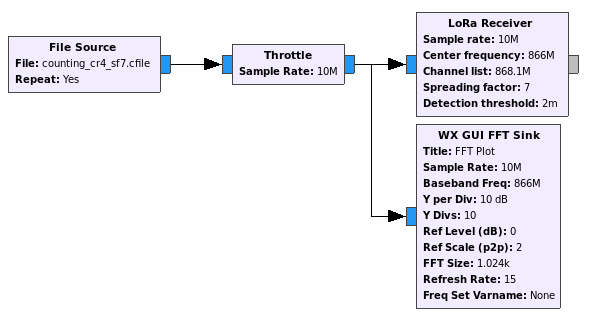
\includegraphics[width=0.8\textwidth]{lora_pic}
 \centering
 \caption{Schemat blokowy GNURadio - odbiornik systemu LoRa.}
\end{figure}


Do odbioru sygnału APRS zostanie wykorzystany odbiornik bazujący na Realtek RTL2832U, pozwalający na bezpośredni przesył strumienia I/Q poprzez złącze USB. Za pomocą sterownika rtl-sdr, sygnał APRS jest traktowany jak źródło dzwięku, które następnie podane na program Xastir pozwala na bezpośredni odbiór wiadomości oraz lokalizację na mapie w czasie rzeczywistym.

\begin{figure}[!htbp]
 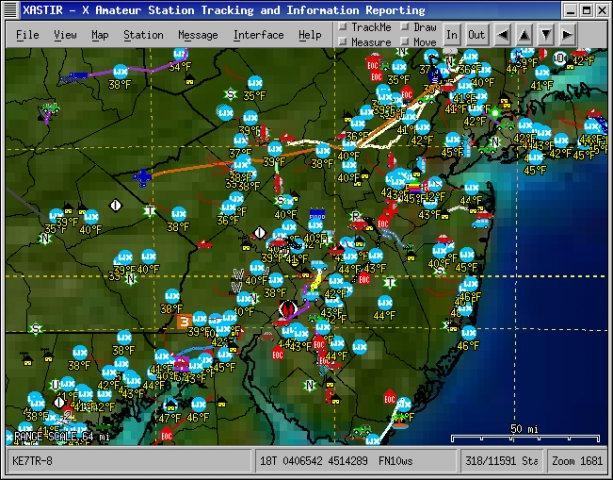
\includegraphics[width=\textwidth]{xastir}
 \centering
 \caption{Widok programu Xastir.}
\end{figure}


Dodatkowo jeden z członków podjął się wykonania części odbiornika na układzie FPGA z przetwornikiem analogowo-cyfrowym. Jest to tylko rozwiązanie cyfrowej demodulacji sygnału, które trzeba uzupełnić o część analogową - filtry i mieszacz. Rozważamy w przyszłości dokończenie tego układu w celu uzyskania bardziej przenośnego rozwiązania i przeniesienia obliczeń na układ FPGA. Na obrazku \ref{fpga} przedstawiono wyniki symulacji demodulatora.


\begin{figure}[!htbp]
 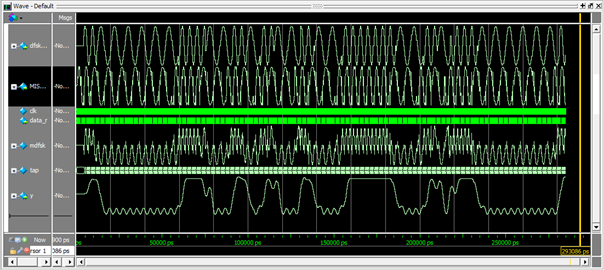
\includegraphics[width=\textwidth]{symulacja}
 \centering
 \caption{Wynik symulacji demodulacji APRS na FPGA}
 \label{fpga}
\end{figure}
% Okazało się, że gotowe projekty oprogramowania demodulatora zarówno APRS jak i LoRa są dostępne w internecie z otwartym oprogramowaniem w GNU radio, więc wystarczyło je przetestować w naszych układach.
